% Belt and pulley system
% Author: Jimi Oke
\documentclass[11pt]{article}
\usepackage{tikz}
\usetikzlibrary{arrows,shapes,positioning,shadows}
\tikzset{
ashadow/.style={opacity=.25, shadow xshift=0.07, shadow yshift=-0.07},
}

\definecolor{CcA}{rgb}{0.2,0.2,0.6}
\definecolor{CcB}{rgb}{0,0,1}
\definecolor{CacA}{rgb}{0.6,0.1,0.1}
\definecolor{CacB}{rgb}{1,0,0}

\tikzset{myxshift/.style = {shift = {(#1, 0)}}}
\tikzset{myyshift/.style = {shift = {(0, #1)}}}

\begin{document}
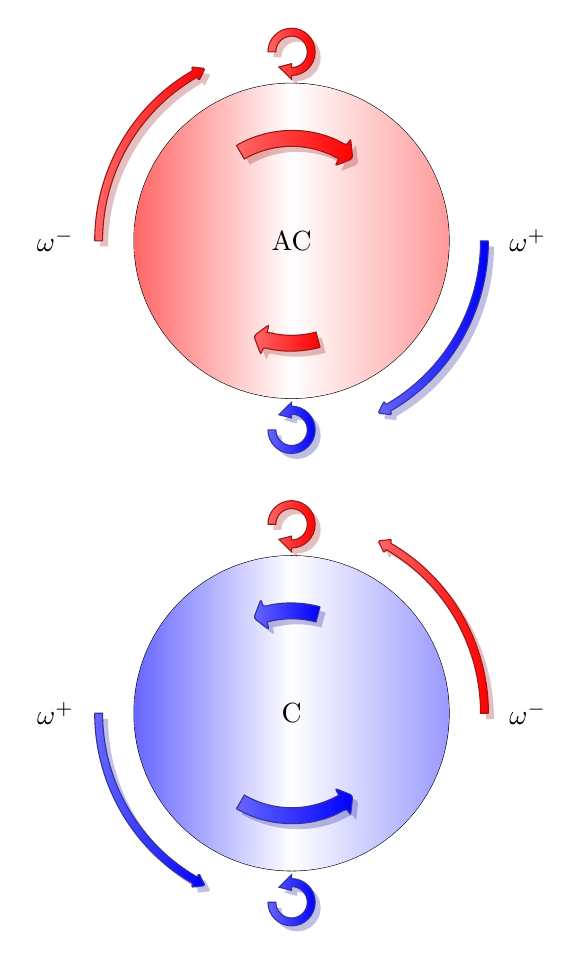
\begin{tikzpicture}
\begin{scope}

%% Definitions
\pgfmathsetmacro{\lenS}{30}
\pgfmathsetmacro{\lenL}{60}
\pgfmathsetmacro{\R}{2}

\newcommand\arrow[5]
{
% arclen: #1
% radius: #2
% thickness: #3
% roundness: #4
% sign: #5
(0:#2+#3)
--
(0:#2)
arc
(0:#5*#1:#2) [rounded corners=#4]
--
(#5*#1:#2-#3/2) [rounded corners=#4]
--
(#5*#1 + #5/#2*2  : #2+#3/2) [rounded corners=#4]
--
(#5*#1:#2+3/2*#3) [rounded corners=#4]
--
(#5*#1:#2+#3)  [rounded corners=#4]
arc
(#5*#1:0:#2+#3) [rounded corners=#4]
}
%%
\newcommand\straightarrow[6]
{
% posX: #1
% posY: #2
% thickness: #3
% roundness: #4
% sign: #5
% len: #6
(#1,#2 + #3/2)
--
(#1,#2 - #3/2)
--
(#1 + #5*#6, #2 - #3/2)
--
(#1 + #5*#6, #2 - #3 )
--
(#1 +#5*#6 +  #5*1, #2  )
--
(#1 + #5*#6, #2 + #3 )
--
(#1 + #5*#6, #2 + #3/2)
--
(#1     , #2 + #3/2)
}
%%
\newcommand\drawACarrow[8]
{
\draw[color=CacA, right color=CacB, left color=CacB!60, drop shadow={ashadow, color=CacB!60!black},myxshift=#7,myyshift=#8] [rotate=#1] \arrow{#2}{#3}{#4}{#5}{#6};
};
%%
\newcommand\drawCarrow[8]
{
\draw[color=CcA, right color=CcB, left color=CcB!60, drop shadow={ashadow, color=CcB!60!black},myxshift=#7,myyshift=#8] [rotate=#1] \arrow{#2}{#3}{#4}{#5}{#6};
};

% --------------------------------------------------------

%%
\newcommand\drawSTRarrow[6]
{
\draw[color=CacA, right color=CacB, left color=CacB!60, drop shadow={ashadow, color=CacB!60!black}]  \straightarrow{#1}{#2}{#3}{#4}{#5}{#6};
};

% --------------------------------------------------------

%% AC

\draw (0,0) circle (\R) ;
\fill[left color=red!60, right color=red!40, middle
color=white] (0,0) circle (\R) ;

\node[] at (0,0) {AC} ;

%  AC - inside - east
\drawACarrow{\lenS/2-90}{\lenS}{0.6*\R}{.2}{1}{-1}{0}{0};
%\node[] at (0:.8*\R) {$\omega^{+}$} ;

%%  AC - inside - west
\drawACarrow{\lenL/2+180-90}{\lenL}{0.6*\R}{.2}{1}{-1}{0}{0};
%\node[] at (180:.8*\R) {$\;\;\omega^{-}$} ;

%  AC - inside - north
%\drawSTRarrow{0}{\lenL}{0.6*\R}{.2}{1}{-1}{0}{0};
%\node[] at (180:.9*\R) {$\;\;\omega^{-}$} ;


%%  AC - outside - east
\drawCarrow{0}{\lenL}{1.2*\R}{.1}{.5}{-1}{0}{0};
\node[] at (0:1.5*\R) {$\omega^{+}$} ;

%%  AC - outside - west
\drawACarrow{180}{\lenL}{1.2*\R}{.1}{.5}{-1}{0}{0};
\node[] at (180:1.5*\R) {$\omega^{-}$} ;

%%  AC - outside - north
\drawACarrow{180}{270}{.1*\R}{.1}{0}{-1}{0}{1.2*\R};

%%  AC - outside - south
\drawCarrow{180}{270}{.1*\R}{.1}{0}{1}{0}{-1.2*\R};


% --------------------------------------------------------

%% C
\draw (0,-3*\R) circle (\R) ;
\fill[left color=blue!60, right color=blue!40, middle
color=white] (0,-3*\R) circle (\R) ;

\node[] at (0,-3*\R) {C} ;

%%  C - inside - east
\drawCarrow{-\lenS/2+90}{\lenS}{0.6*\R}{.2}{1}{1}{0}{-3*\R};
%\node[myyshift=-3*\R] at (0:.8*\R) {$\omega^{-}$} ;

%%  C - inside - west
\drawCarrow{-\lenL/2+180+90}{\lenL}{0.6*\R}{.2}{1}{1}{0}{-3*\R};
%\node[myyshift=-3*\R] at (180:.8*\R) {$\;\;\omega^{+}$} ;

%%  C - outside - east
\drawACarrow{0}{\lenL}{1.2*\R}{.1}{.5}{1}{0}{-3*\R};
\node[myyshift=-3*\R] at (0:1.5*\R) {$\omega^{-}$} ;

%%  C - outside - west
\drawCarrow{180}{\lenL}{1.2*\R}{.1}{.5}{1}{0}{-3*\R};
\node[myyshift=-3*\R] at (180:1.5*\R) {$\omega^{+}$} ;

%%  C - outside - north
\drawACarrow{180}{270}{.1*\R}{.1}{0}{-1}{0}{-3*\R + 1.2*\R};

%%  C - outside - south
\drawCarrow{180}{270}{.1*\R}{.1}{0}{1}{0}{-3*\R + -1.2*\R};


% --------------------------------------------------------



%\shade[ball color=white] (0,0) circle (.3) node[left,xshift=-5] {$P$};
%\draw[thick, white] (0,0) circle (.8*\R);
% Pulleys

%% big pulley
%\draw (0,0) circle (\R) ;
%\fill[left color=gray!80, right color=gray!60, middle
%color=white] (0,0) circle (\R) ;
%\draw[thick, white] (0,0) circle (.8*\R);
%\shade[ball color=white] (0,0) circle (.3) node[left,xshift=-5] {$P$};

%% small pulley
%\draw (\Q+\q-.3, 0) circle (\r);
%\fill[left color=gray!80, right color=gray!60, middle
%color=white] (\Q+\q-.3, 0) circle (\r) ;
%\draw[thick, white] (\Q+\q-.3,0) circle (.8*\r);
%\shade[ball color=white] (\Q+\q-.3,0) circle (.15) 
%node[right, xshift=2] {$Q$};

% belt and point labels
%\begin{scope}[ultra thick]
%\draw (\b:\R) arc (\b:360-\b:\R) ;
%\draw (\b:\R) -- ( \P, 0 ); 
%\draw (-\b:\R) -- ( \P, 0 );
%\draw (\Q-.3,0) -- + (\a:\p)  arc (105:-105:\r) ;
%\draw (\Q-.3,0) -- + (-\a:\p);
%%\draw (\b:\R) arc (\b:360-\b:\r) ;
%\end{scope}

%\draw (0,0) -- (\b:\R) node[midway, above,sloped] {$R$} node[above] {$A$};
%\draw (-\b:\R)--(0,0) ;
%\draw (\Q+\q-.3,0) -- +(105:\r) node[midway,above, sloped] {$r$}
%node[above] {$E$};
%\draw (\Q+\q-.3,0) -- +(-105:\r) node[below] {$D$};
%\node[below] at (-\b:\R) {$B$};
%\node[below] at (\Q-.3,0) {$C$};

%% center line
%\draw[dash pattern=on5pt off3pt] (0,0) -- (\Q+\q-.3,0);

%% angle label
%\draw (\Q-1.8,0) arc (180:195:1.5);
%\draw (\Q-1.8,0) arc (180:165:1.5);
\end{scope}
\end{tikzpicture}
\end{document} 
